\documentclass[10pt,twocolumn]{article}

\usepackage[margin=0.75in]{geometry}
\usepackage[T1]{fontenc}
\usepackage[utf8]{inputenc}
\usepackage{lmodern}
\usepackage{microtype}
\usepackage{amsmath,amssymb,amsfonts}
\usepackage{booktabs}
\usepackage{graphicx}
\usepackage{subcaption}
\usepackage{float}
\usepackage{multirow}
\usepackage{enumitem}
\usepackage{hyperref}
\usepackage{xcolor}
\usepackage{mathtools}

\hypersetup{
  colorlinks=true,
  linkcolor=blue,
  urlcolor=blue,
  citecolor=blue
}

\title{\bf A Toy-2D Study of Diffusion Posterior Sampling and\\Flow with Interpolant Guidance for Linear Inverse Problems}
\author{Project report extending the original FIG repository with a dedicated toy-2D benchmark}
\date{March 2026}

\begin{document}
\maketitle

\begin{abstract}
This paper presents a complete toy-2D benchmark for comparing Diffusion Posterior Sampling (DPS), plain Flow with Interpolant Guidance (FIG), and FIG+ on linear inverse problems. The study extends the original FIG GitHub repository, which primarily targets image restoration, with a low-dimensional experimental pipeline designed for direct geometric inspection of the posterior. In the final version of the benchmark, the diffusion prior is modeled by a residual, time-conditioned DDPM denoiser trained from scratch with exponential moving average (EMA) weights. This improved prior substantially strengthens the unconditional fit on both Two-Moons and Eight-Gaussians and makes the conditional comparison more informative. Across the reported experiments, FIG+ is consistently the strongest method on posterior-quality metrics, while plain FIG remains unstable and DPS becomes sensitive to guidance strength in the most constrained regimes. The toy setting remains the main asset of the study: one can visualize the prior manifold, the observation line, the reference posterior, and the full denoising trajectories of the competing samplers.
\end{abstract}

\section{Introduction}

Diffusion-based priors have become a powerful tool for inverse problems, but their behavior is often difficult to interpret in image space. Conditional samplers can fail for several intertwined reasons: the prior may be underfit, the sampler may be too deterministic, the conditioning gradient may be mis-scaled, or the target posterior may simply be highly multimodal. This motivates a deliberately low-dimensional benchmark where every element of the problem is visible.

The present work was developed in the context of the original \textit{Flow with Interpolant Guidance} (FIG) repository. That repository implements diffusion- and flow-based inverse-problem solvers for image tasks such as super-resolution, deblurring, and inpainting. Our goal here is complementary: rather than reproducing the full image pipeline, we construct a self-contained 2D environment in which the geometry of DPS, FIG, and FIG+ can be inspected directly.

The resulting benchmark answers three questions:
\begin{enumerate}[leftmargin=1.5em]
    \item Can a compact DDPM prior trained from scratch recover non-Gaussian toy distributions such as Two-Moons and Eight-Gaussians?
    \item How do DPS, plain FIG, and FIG+ behave under a one-dimensional noisy linear observation?
    \item How much of the final behavior comes from the prior itself, and how much comes from the conditional solver?
\end{enumerate}

\section{Extension of the Original Repository}

The upstream FIG repository is centered on image inverse problems with strong pretrained priors. It does not provide a dedicated 2D experimental environment. We therefore added the following components:
\begin{itemize}[leftmargin=1.5em]
    \item synthetic data generators for \texttt{two\_moons} and \texttt{eight\_gaussians};
    \item a DDPM training pipeline for 2D priors;
    \item a residual, time-conditioned MLP denoiser with EMA checkpointing;
    \item a linear inverse-problem module with Gaussian measurement noise;
    \item toy implementations of DPS, FIG, and FIG+;
    \item a reference posterior sampler based on importance reweighting of exact prior samples;
    \item evaluation scripts exporting CSV summaries, plots, and denoising animations.
\end{itemize}

This extension turns the original repository into a testbed where the conditioning mechanism can be examined independently of image-scale architectural complexity.

\section{Problem Setup}

\subsection{Toy Distributions}

We consider two standard non-Gaussian toy datasets:
\begin{itemize}[leftmargin=1.5em]
    \item \textbf{Two-Moons}, a curved bimodal manifold that is useful for studying conditional sampling on nonlinear supports;
    \item \textbf{Eight-Gaussians}, a strongly multimodal distribution arranged on a ring, well suited to diagnosing mode preservation.
\end{itemize}

\subsection{Improved Diffusion Prior}

For each dataset, we train a DDPM prior from scratch. The forward process is
\begin{equation}
\mathbf{x}_t = \sqrt{\bar{\alpha}_t}\,\mathbf{x}_0 + \sqrt{1-\bar{\alpha}_t}\,\boldsymbol{\epsilon},
\qquad
\boldsymbol{\epsilon} \sim \mathcal{N}(\mathbf{0}, I),
\end{equation}
and the denoiser predicts \(\boldsymbol{\epsilon}_\theta(\mathbf{x}_t,t)\) by minimizing
\begin{equation}
\mathcal{L}_{\mathrm{DDPM}}
=
\mathbb{E}_{\mathbf{x}_0, t, \boldsymbol{\epsilon}}
\left[
\left\|
\boldsymbol{\epsilon} - \boldsymbol{\epsilon}_\theta(\mathbf{x}_t,t)
\right\|_2^2
\right].
\end{equation}

The final denoiser architecture is a residual, time-conditioned MLP. This choice is intentional:
\begin{itemize}[leftmargin=1.5em]
    \item the data lives in \(\mathbb{R}^2\), so a U-Net would be unnecessary and would not exploit any meaningful spatial hierarchy;
    \item sinusoidal timestep embeddings provide a rich representation of the diffusion time;
    \item a small time MLP projects those embeddings into the hidden state dimension;
    \item each residual block applies LayerNorm, then a time-dependent scale-shift modulation, then a two-layer SiLU MLP;
    \item residual connections stabilize deeper networks and help preserve multimodal structure;
    \item an EMA of the weights is maintained during training and used for sampling.
\end{itemize}

This architecture is substantially stronger than the original plain MLP baseline. In practice, it solves two issues that were visible in earlier experiments: underfitting of Eight-Gaussians, and poor mode coverage under deterministic sampling.

The reported runs use \(128\) diffusion steps, a cosine schedule, \(6000\) optimization steps, batch size \(1024\), hidden dimension \(256\), time embedding dimension \(128\), \(6\) residual blocks, learning rate \(3\times 10^{-4}\), and EMA decay \(0.995\).

\begin{figure*}[t]
    \centering
    \begin{subfigure}{0.49\textwidth}
        \centering
        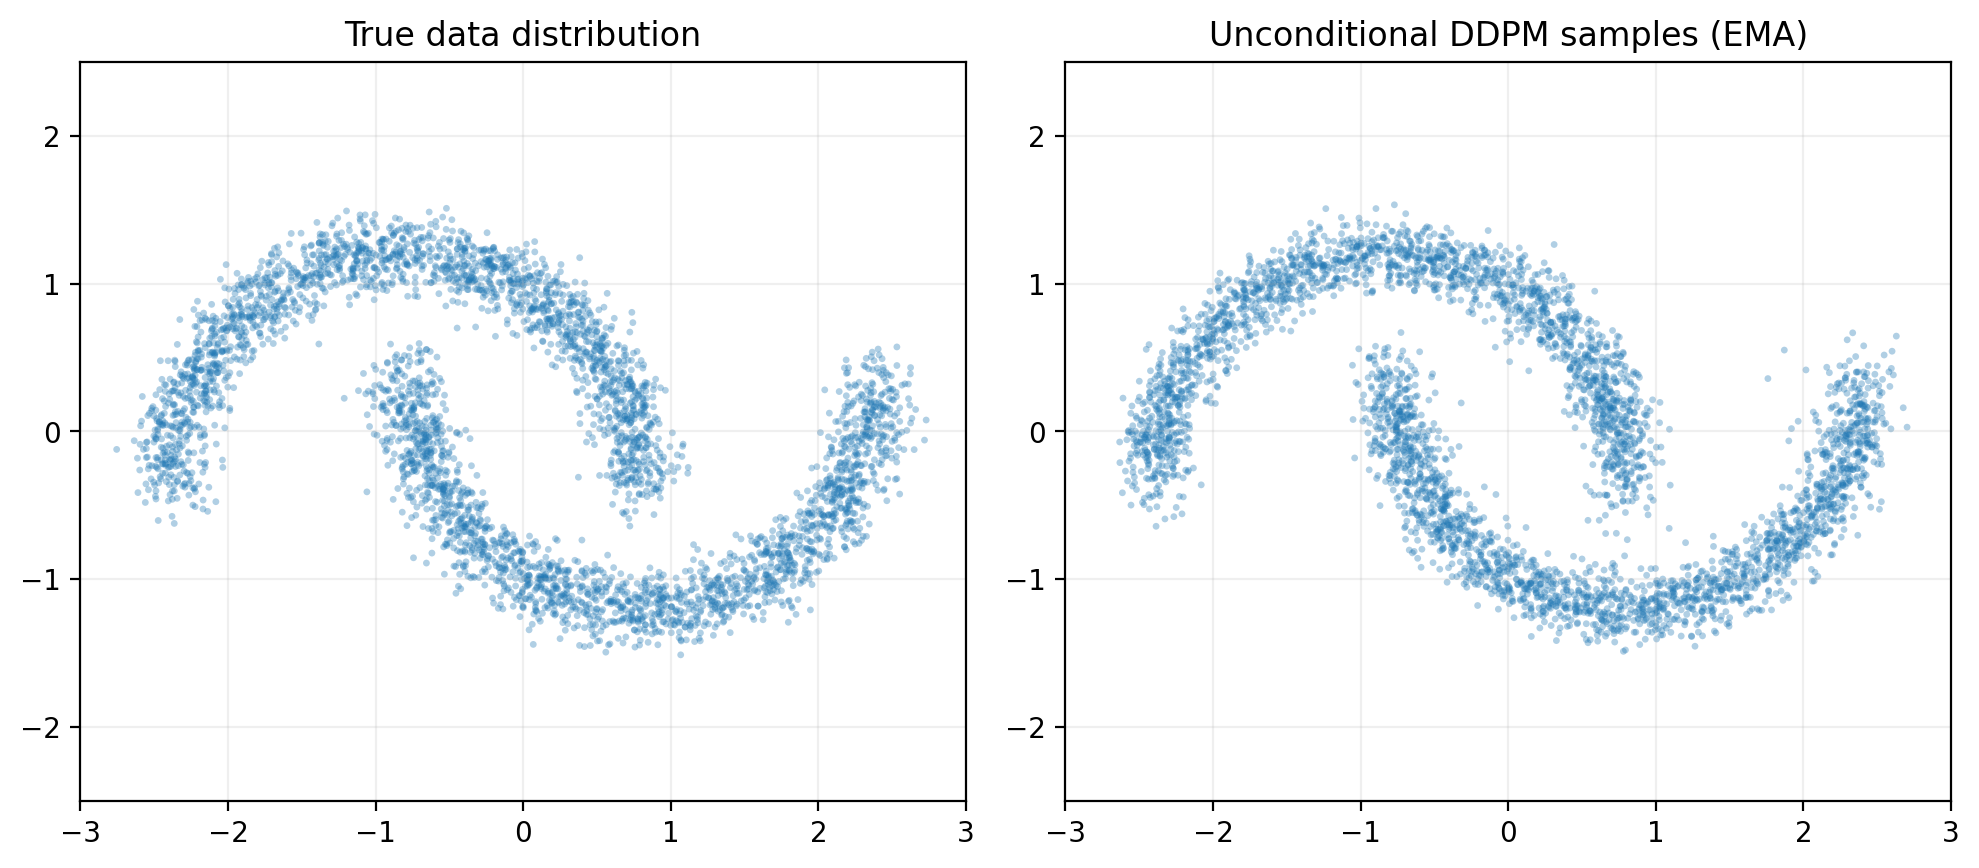
\includegraphics[width=\textwidth]{report_assets/two_moons_unconditional_check.png}
        \caption{Two-Moons prior sanity check.}
    \end{subfigure}
    \hfill
    \begin{subfigure}{0.49\textwidth}
        \centering
        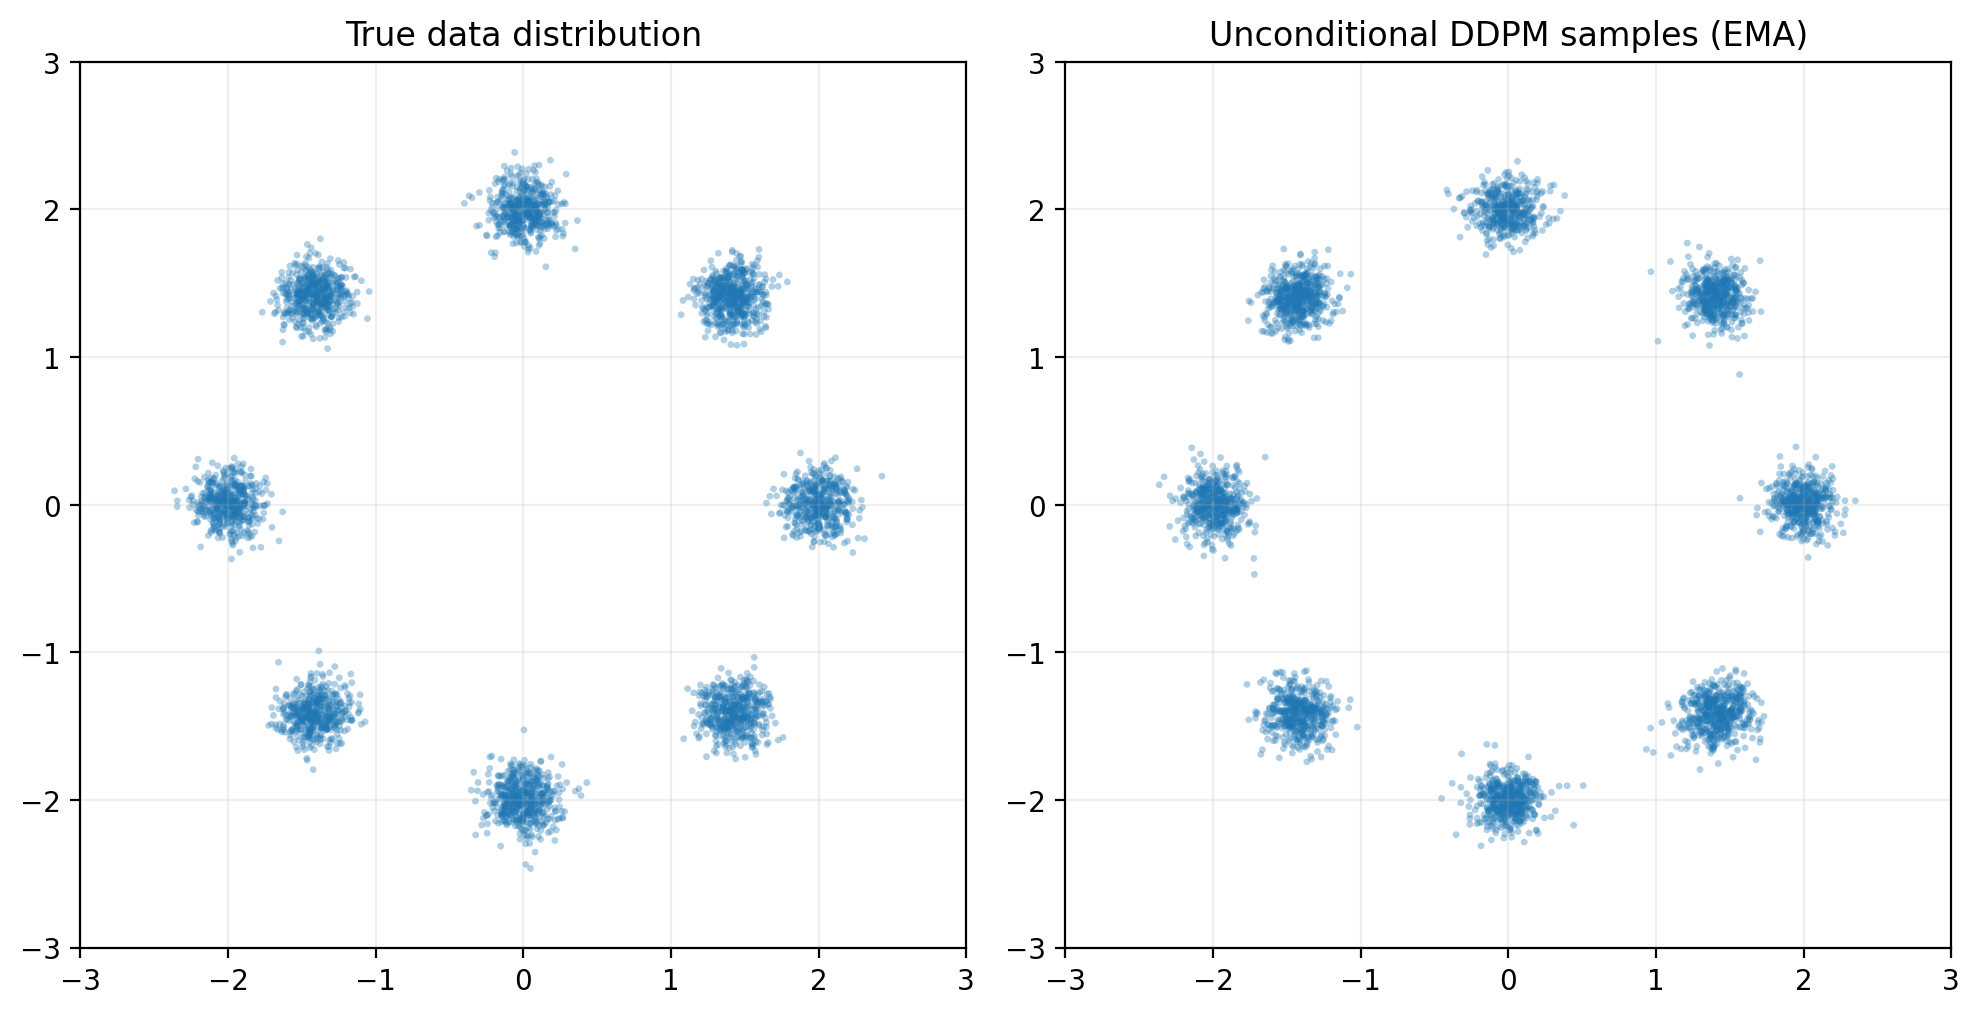
\includegraphics[width=\textwidth]{report_assets/eight_gaussians_unconditional_check.png}
        \caption{Eight-Gaussians prior sanity check.}
    \end{subfigure}
    \caption{Unconditional prior checks obtained with ancestral DDPM sampling and EMA weights. The improved denoiser recovers the global geometry of both toy distributions, which makes the subsequent conditional comparison more meaningful.}
    \label{fig:prior_checks}
\end{figure*}

For unconditional sanity checks we use an ancestral DDPM sampler rather than a deterministic DDIM sampler. This matters in low dimension: DDIM can visually underrepresent multimodality even when the underlying denoiser is already good. For the inverse-problem solvers themselves, we keep the DDIM backbone so that DPS, FIG, and FIG+ are compared under the same deterministic reverse trajectory.

\subsection{Linear Inverse Problem}

We study the noisy linear observation model
\begin{equation}
\mathbf{y} = A\mathbf{x}^\star + \mathbf{n},
\qquad
A = \begin{bmatrix}1 & 0\end{bmatrix},
\qquad
\mathbf{n} \sim \mathcal{N}(\mathbf{0}, \sigma_n^2 I).
\end{equation}

Hence, the first coordinate is observed while the second coordinate remains hidden. This is the 2D analogue of a mask-like inpainting operator: the posterior is supported on the vertical line \(x_1 = y\), but the distribution along that line remains structured because the prior is non-Gaussian.

\subsection{Reference Posterior and Metrics}

To evaluate the samplers against a meaningful target, we approximate the conditional posterior with importance reweighting. A large pool of exact prior samples \(\{\mathbf{x}^{(i)}\}_{i=1}^N\) is drawn from the true toy distribution, and the weights
\begin{equation}
w_i \propto \exp\left(
-\frac{\|A\mathbf{x}^{(i)} - \mathbf{y}\|_2^2}{2\sigma_n^2}
\right)
\end{equation}
define an empirical approximation of \(p(\mathbf{x}\mid \mathbf{y})\).

We report:
\begin{itemize}[leftmargin=1.5em]
    \item \textbf{Posterior Mean MSE}: error between the mean of generated samples and the mean of the reference posterior;
    \item \textbf{Sliced Wasserstein Distance (SWD)}: discrepancy between the generated and reference conditional distributions;
    \item \textbf{Measurement MSE}: average \(\|A\mathbf{x} - \mathbf{y}\|_2^2\), which quantifies measurement consistency.
\end{itemize}

\section{Conditional Solvers}

\subsection{Diffusion Posterior Sampling}

DPS uses Tweedie's formula to estimate the clean sample
\begin{equation}
\hat{\mathbf{x}}_0
=
\frac{
\mathbf{x}_t - \sqrt{1-\bar{\alpha}_t}\,\boldsymbol{\epsilon}_\theta(\mathbf{x}_t,t)
}{
\sqrt{\bar{\alpha}_t}
}.
\end{equation}
It then evaluates the measurement loss
\begin{equation}
\mathcal{L}_{\mathrm{meas}}^{\mathrm{DPS}}
=
\left\|
\mathbf{y} - A\hat{\mathbf{x}}_0
\right\|_2^2
\end{equation}
and backpropagates that loss to the current noisy state before taking the unconditional DDIM update.

\subsection{Plain FIG}

FIG introduces a measurement interpolant
\begin{equation}
\mathbf{y}_{t-1}
=
\sqrt{\bar{\alpha}_{t-1}}\,\mathbf{y}
+
w\sqrt{1-\bar{\alpha}_{t-1}}\,A\boldsymbol{\epsilon},
\end{equation}
with \(\boldsymbol{\epsilon}\sim\mathcal{N}(\mathbf{0}, I)\), then applies \(K\) gradient steps to the Gaussian negative log-likelihood
\begin{equation}
\mathcal{L}_{\mathrm{meas}}^{\mathrm{FIG}}
=
\frac{1}{2\sigma_n^2}
\left\|
\mathbf{y}_{t-1} - A\mathbf{x}
\right\|_2^2.
\end{equation}

In our implementation, the conditional step is scaled with a noise-dependent factor inspired by the SNR interpretation of FIG:
\begin{equation}
\eta_{t-1}
=
c\,\Delta t\,
\frac{1-\bar{\alpha}_{t-1}}{\bar{\alpha}_{t-1}\,\|A\|_2^2},
\qquad
\Delta t = \frac{1}{T}.
\end{equation}
This provides a practical DDPM-compatible analogue of the theoretical FIG scaling.

\subsection{FIG+ for Mask-Like Operators}

Because the operator \(A=[1,0]\) acts like a coordinate mask, we also study FIG+, which mixes the hidden coordinate with a Tweedie-based estimate. After computing \(\hat{\mathbf{x}}_0\), we perturb it back to the next time level,
\begin{equation}
\tilde{\mathbf{x}}_{t-1}
=
\sqrt{\bar{\alpha}_{t-1}}\,\hat{\mathbf{x}}_0
+
\sqrt{1-\bar{\alpha}_{t-1}}\,\boldsymbol{\epsilon},
\end{equation}
and combine it with the updated state through
\begin{equation}
\mathbf{x}_{t-1}
\leftarrow
P\mathbf{x}_{t-1}
+
(1-m)(I-P)\mathbf{x}_{t-1}
+
m(I-P)\tilde{\mathbf{x}}_{t-1},
\end{equation}
where \(P=\mathrm{diag}(1,0)\) selects the observed coordinate and \(m\in[0,1]\) is a mixing coefficient. Intuitively, this keeps the observed coordinate measurement-consistent while restoring diversity in the hidden component.

\section{Experimental Protocol}

The evaluation is performed on both toy datasets with measurement noise levels
\[
\sigma_n \in \{0.05, 0.5, 1.0\}.
\]
For each dataset and each noise level, we use:
\begin{itemize}[leftmargin=1.5em]
    \item \(6\) test observations;
    \item \(128\) conditional samples per solver and per observation;
    \item \(128\) reference posterior samples;
    \item a \(20{,}000\)-sample importance pool for posterior approximation.
\end{itemize}

For plain FIG and FIG+, we ablate
\[
K \in \{1,3,5\},
\qquad
w \in \{0.0, 0.5\}.
\]
We keep the solver hyperparameters fixed across datasets: DPS uses \(\zeta=0.05\), FIG and FIG+ use learning rate \(0.5\), and FIG+ uses mixing coefficient \(m=0.95\).

\section{Results}

\subsection{Quantitative Results on Two-Moons}

\begin{table*}[t]
\centering
\small
\caption{Two-Moons results with the improved residual DDPM prior. Lower is better for all metrics.}
\begin{tabular}{lccccc}
\toprule
\(\sigma_n\) & Solver & Best \((K,w)\) & Posterior Mean MSE & SWD & Measurement MSE \\
\midrule
0.05 & DPS & -- & \(2.14\times 10^{-2}\) & 0.314 & \(2.40\times 10^{-3}\) \\
0.05 & FIG & (5, 0.0) & \(8.86\times 10^{1}\) & 51.804 & \(5.93\times 10^{-3}\) \\
0.05 & FIG+ & (5, 0.5) & \(2.23\times 10^{-2}\) & 0.212 & \(5.65\times 10^{-3}\) \\
\midrule
0.50 & DPS & -- & \(2.70\times 10^{1}\) & 39.698 & \(1.21\) \\
0.50 & FIG & (5, 0.0) & \(4.01\) & 38.656 & \(1.11\times 10^{-1}\) \\
0.50 & FIG+ & (5, 0.5) & \(1.77\times 10^{-2}\) & 0.314 & \(2.29\times 10^{-2}\) \\
\midrule
1.00 & DPS & -- & \(9.17\) & 21.189 & \(6.79\times 10^{-4}\) \\
1.00 & FIG & (5, 0.0) & \(3.84\) & 35.032 & \(3.51\times 10^{-1}\) \\
1.00 & FIG+ & (5, 0.0) & \(1.90\times 10^{-2}\) & 0.508 & \(7.35\times 10^{-2}\) \\
\bottomrule
\end{tabular}
\label{tab:two_moons}
\end{table*}

\begin{figure*}[t]
    \centering
    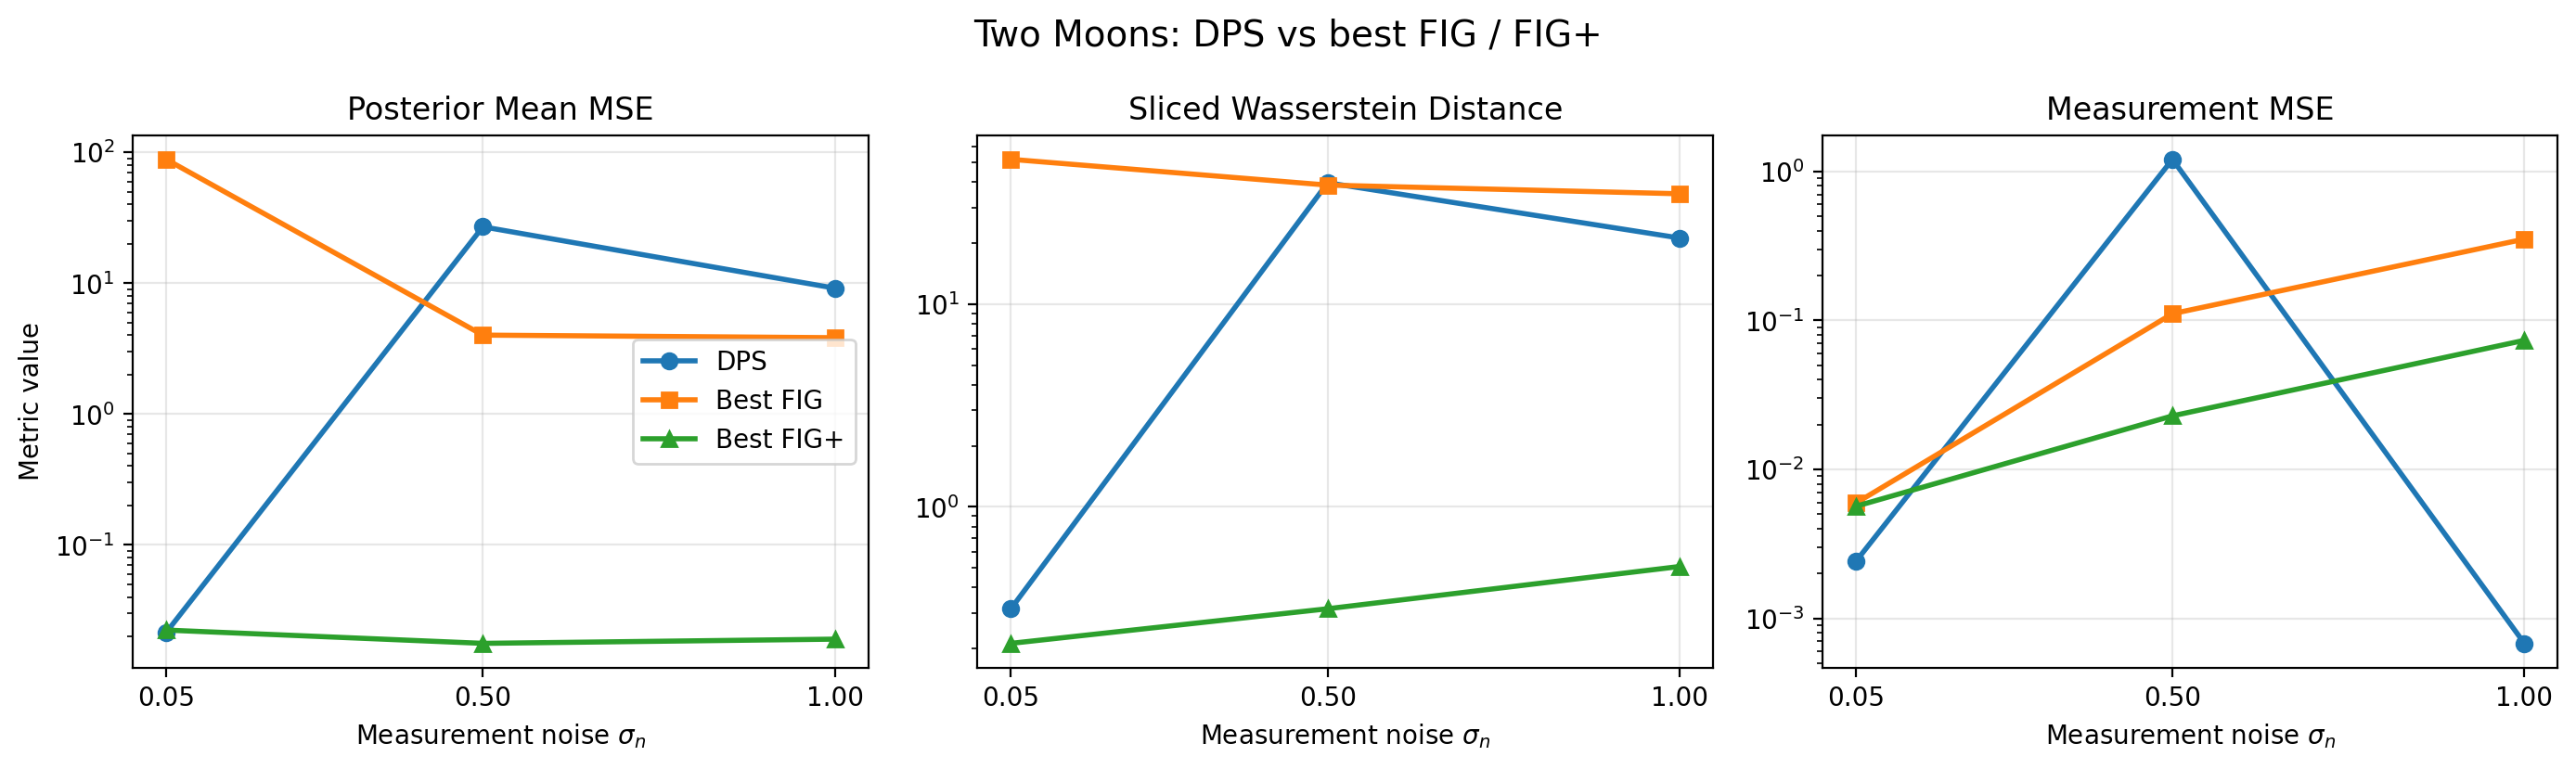
\includegraphics[width=\textwidth]{report_assets/two_moons_paper_metric_trends.png}
    \caption{Two-Moons quantitative trends with the improved prior. FIG+ dominates the posterior-quality metrics across all tested noise levels. Plain FIG remains unstable, while DPS becomes highly sensitive to the guidance strength once the posterior becomes sharply concentrated.}
    \label{fig:two_moons_trends}
\end{figure*}

With the stronger prior in place, the main bottleneck is no longer unconditional generation. The comparison now isolates the conditional solvers more clearly. On Two-Moons, FIG+ is the only method that stays close to the reference posterior across all noise levels. DPS is competitive at very low noise but becomes unstable at \(\sigma_n=0.5\) and \(\sigma_n=1.0\) under the fixed \(\zeta\) used here, while plain FIG fails to preserve the bimodal posterior geometry.

\subsection{Quantitative Results on Eight-Gaussians}

\begin{table*}[t]
\centering
\small
\caption{Eight-Gaussians results with the improved residual DDPM prior. Lower is better for all metrics.}
\begin{tabular}{lccccc}
\toprule
\(\sigma_n\) & Solver & Best \((K,w)\) & Posterior Mean MSE & SWD & Measurement MSE \\
\midrule
0.05 & DPS & -- & \(1.51\) & 10.209 & \(9.57\times 10^{1}\) \\
0.05 & FIG & (5, 0.5) & \(1.27\times 10^{2}\) & 28.956 & \(3.04\times 10^{-2}\) \\
0.05 & FIG+ & (5, 0.5) & \(1.91\times 10^{-2}\) & 0.430 & \(2.19\times 10^{-2}\) \\
\midrule
0.50 & DPS & -- & \(5.85\times 10^{-2}\) & 2.043 & \(7.45\times 10^{-3}\) \\
0.50 & FIG & (5, 0.0) & \(2.91\) & 23.242 & \(2.23\times 10^{-1}\) \\
0.50 & FIG+ & (5, 0.0) & \(1.17\times 10^{-2}\) & 0.320 & \(8.54\times 10^{-2}\) \\
\midrule
1.00 & DPS & -- & \(1.11\times 10^{-1}\) & 1.409 & \(2.97\times 10^{-3}\) \\
1.00 & FIG & (5, 0.0) & \(1.31\) & 11.759 & \(3.33\times 10^{-1}\) \\
1.00 & FIG+ & (5, 0.0) & \(4.21\times 10^{-2}\) & 0.635 & \(9.30\times 10^{-2}\) \\
\bottomrule
\end{tabular}
\label{tab:eight_gaussians}
\end{table*}

\begin{figure*}[t]
    \centering
    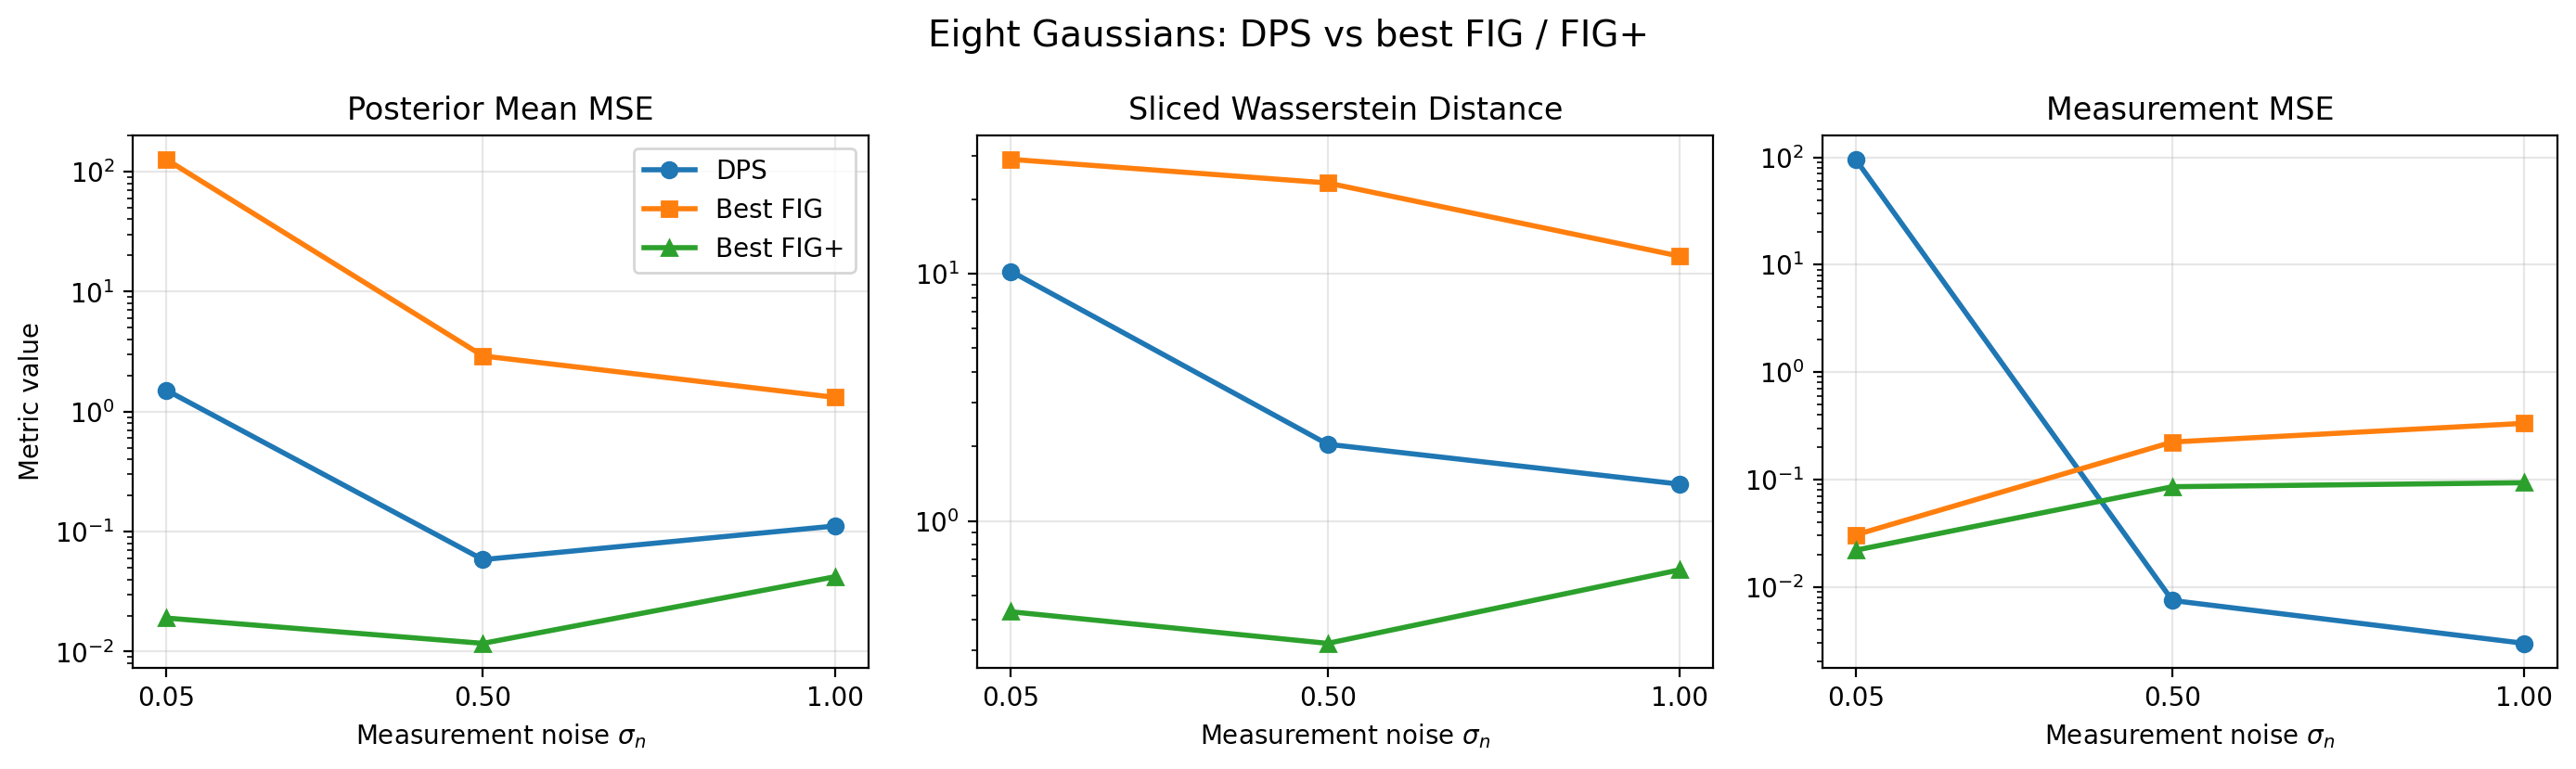
\includegraphics[width=\textwidth]{report_assets/eight_gaussians_paper_metric_trends.png}
    \caption{Eight-Gaussians quantitative trends with the improved prior. FIG+ again provides the best posterior fit. DPS remains competitive at moderate and high measurement noise, but deteriorates sharply at low measurement noise where the posterior is highly multimodal and tightly constrained.}
    \label{fig:eight_trends}
\end{figure*}

Eight-Gaussians makes the mode-preservation issue even clearer. Because several clusters remain plausible under a fixed observed first coordinate, the solver must preserve multimodality rather than simply collapse toward a narrow line. FIG+ is consistently the strongest method of the three. DPS remains reasonable for \(\sigma_n \in \{0.5, 1.0\}\), but becomes unreliable for \(\sigma_n=0.05\), where the posterior is both tight and multimodal.

\subsection{Inpainting Dynamics Along Fixed Observation Lines}

Static metrics only show the endpoint of the solver. To inspect the conditioning mechanism itself, we generated denoising animations from a shared Gaussian initialization for two fixed observation lines, \(x_1=0\) and \(x_1=1\), on both datasets. These four cases are particularly informative because they correspond to different posterior geometries: ambiguous symmetric conditioning at \(x_1=0\), and more asymmetric conditioning at \(x_1=1\).

\begin{figure*}[t]
    \centering
    \begin{subfigure}{0.49\textwidth}
        \centering
        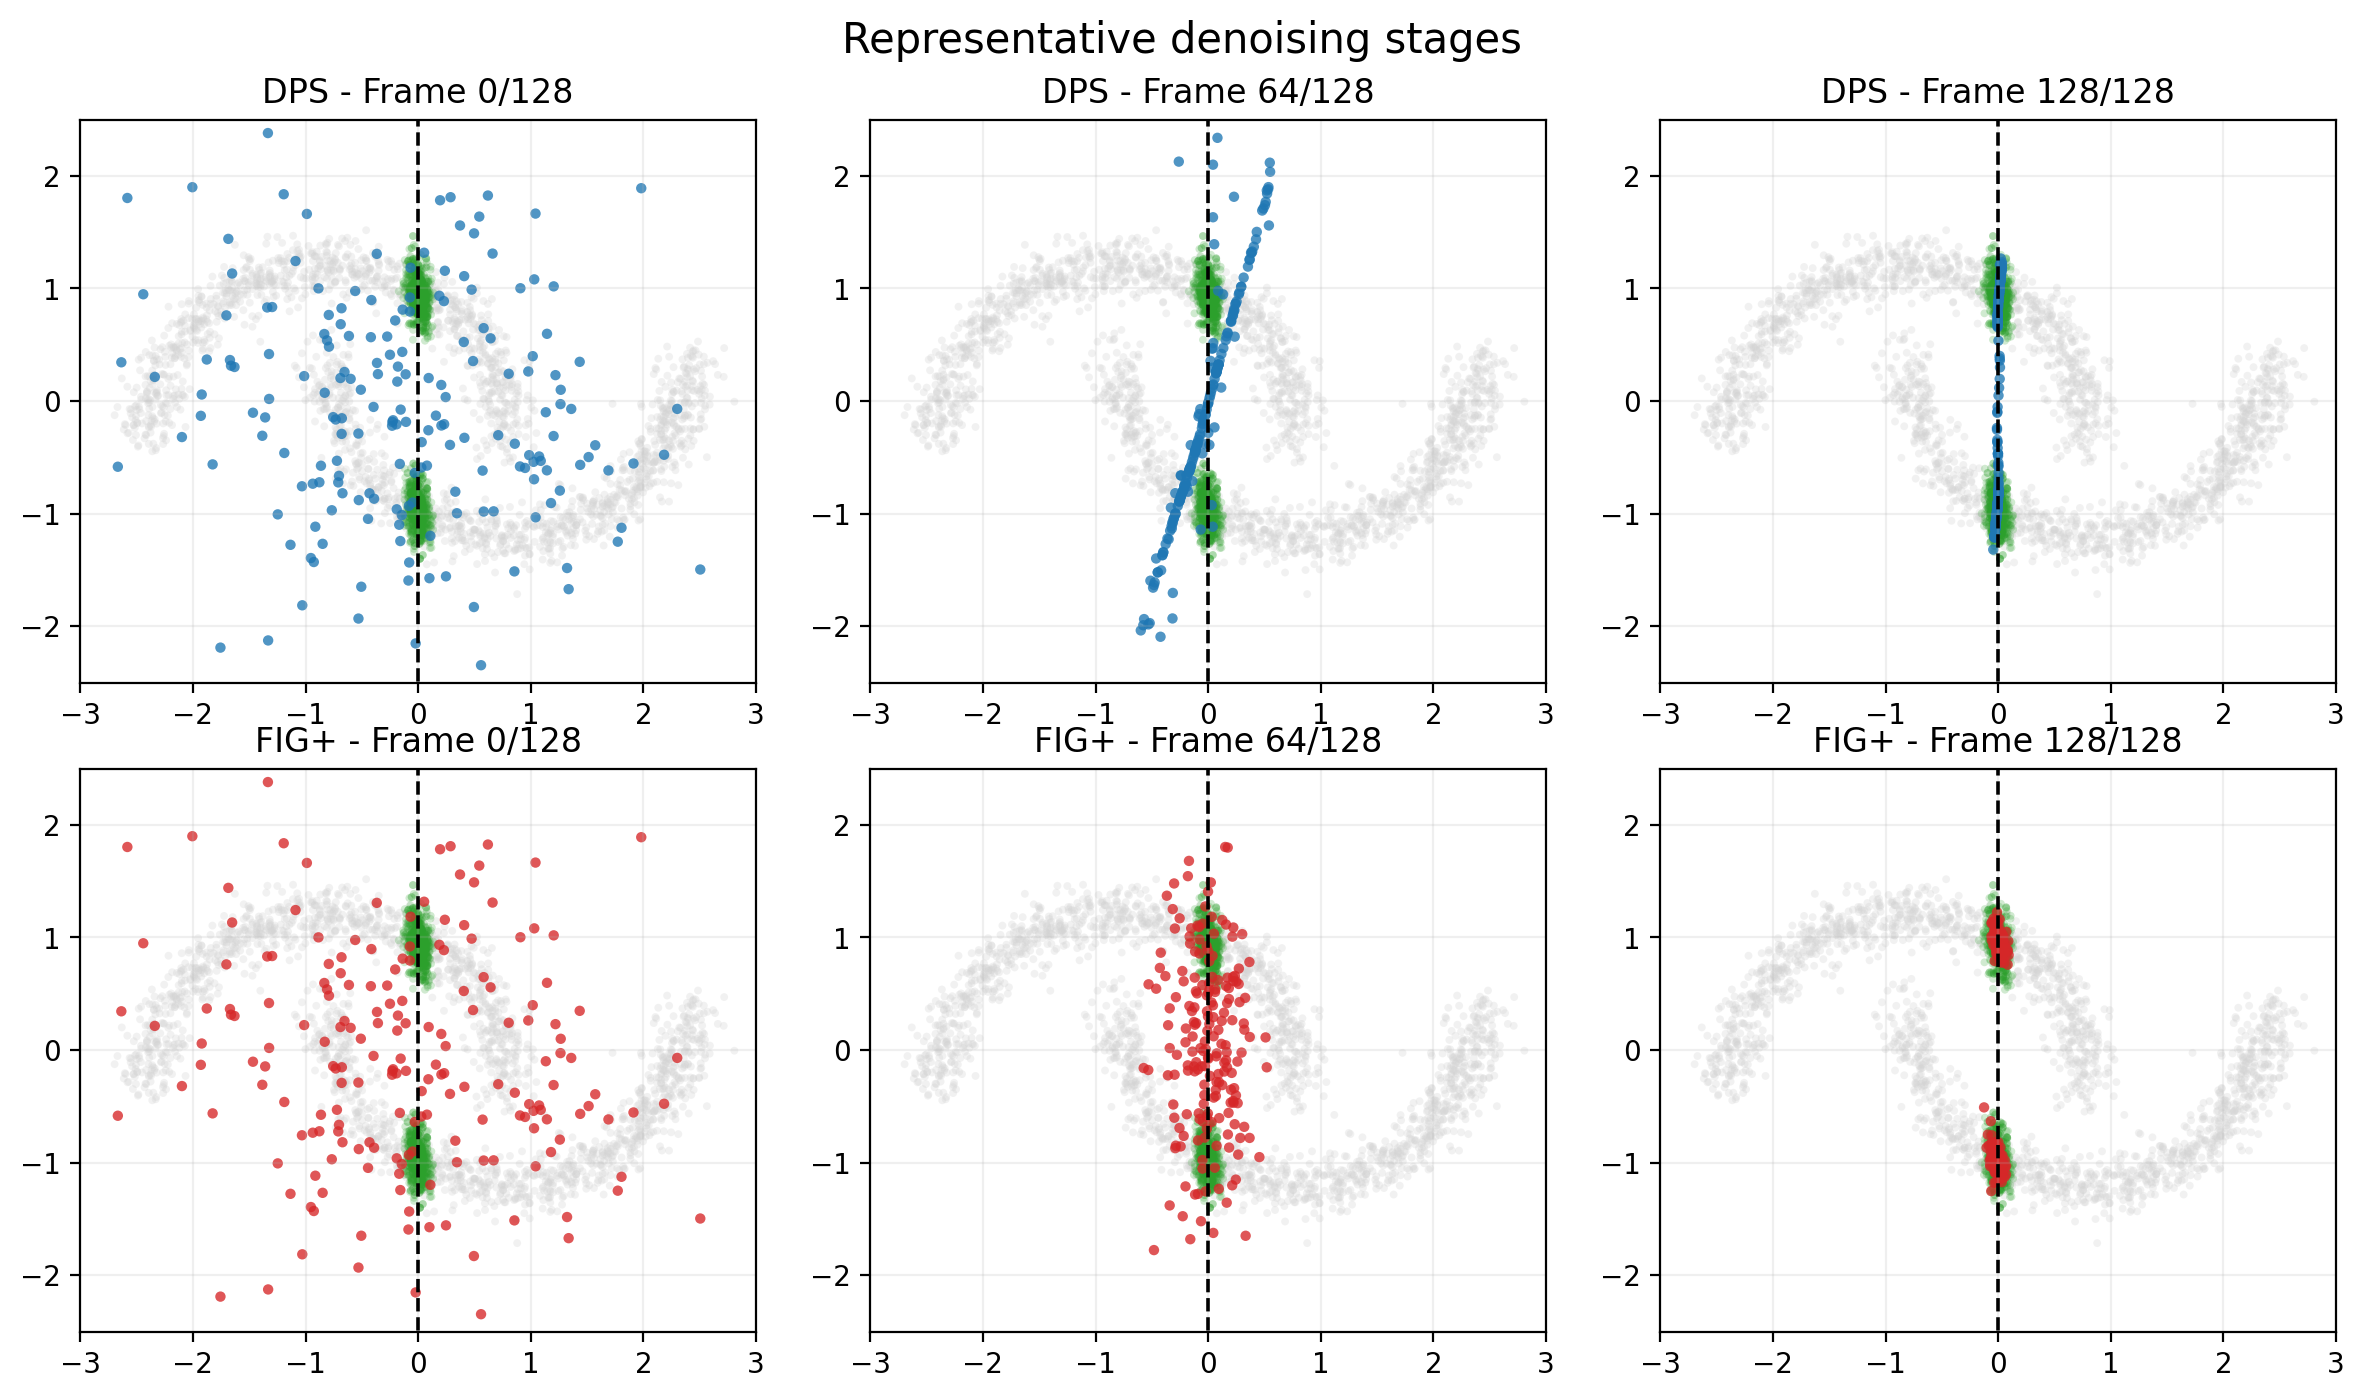
\includegraphics[width=\textwidth]{animations/two_moons_sigma_0.05_x1_p0.00_vs_dps_vs_fig_plus_strip.png}
        \caption{Two-Moons, fixed line \(x_1 = 0\).}
    \end{subfigure}
    \hfill
    \begin{subfigure}{0.49\textwidth}
        \centering
        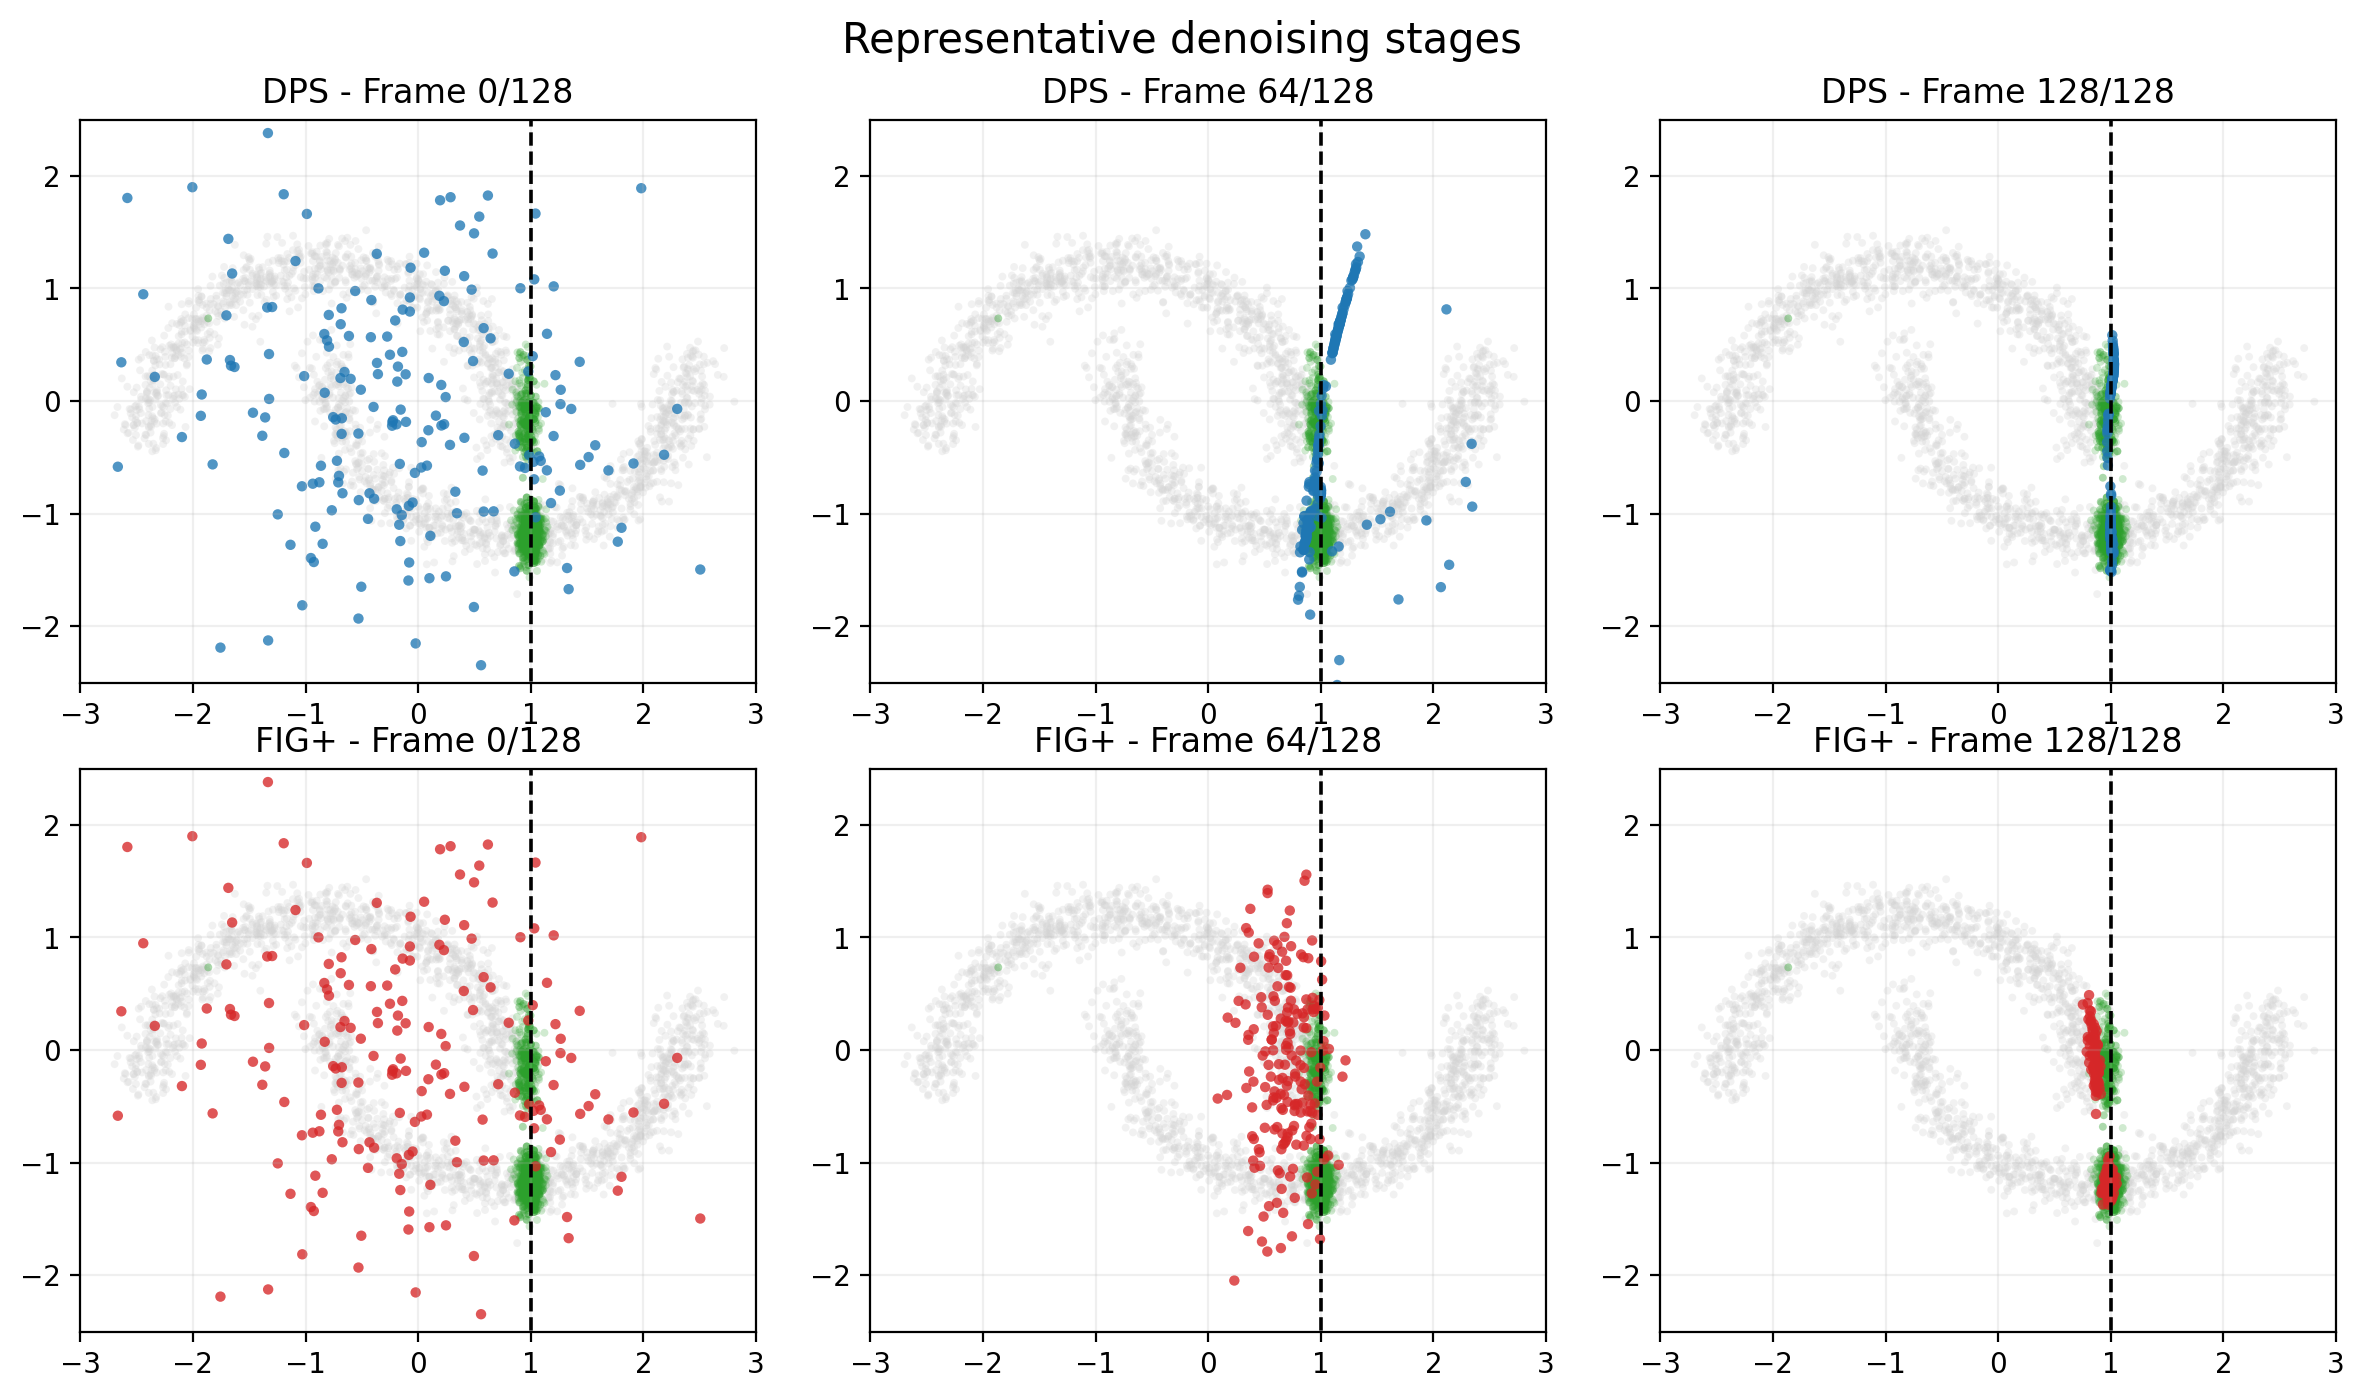
\includegraphics[width=\textwidth]{animations/two_moons_sigma_0.05_x1_p1.00_vs_dps_vs_fig_plus_strip.png}
        \caption{Two-Moons, fixed line \(x_1 = 1\).}
    \end{subfigure}
    \caption{Representative denoising stages for Two-Moons. Gray denotes the true prior support, green denotes the reference posterior, blue denotes DPS, and red denotes FIG+. FIG+ reaches the correct modes more directly and with less residual spread away from the observation line.}
    \label{fig:two_moons_dynamics}
\end{figure*}

\begin{figure*}[t]
    \centering
    \begin{subfigure}{0.49\textwidth}
        \centering
        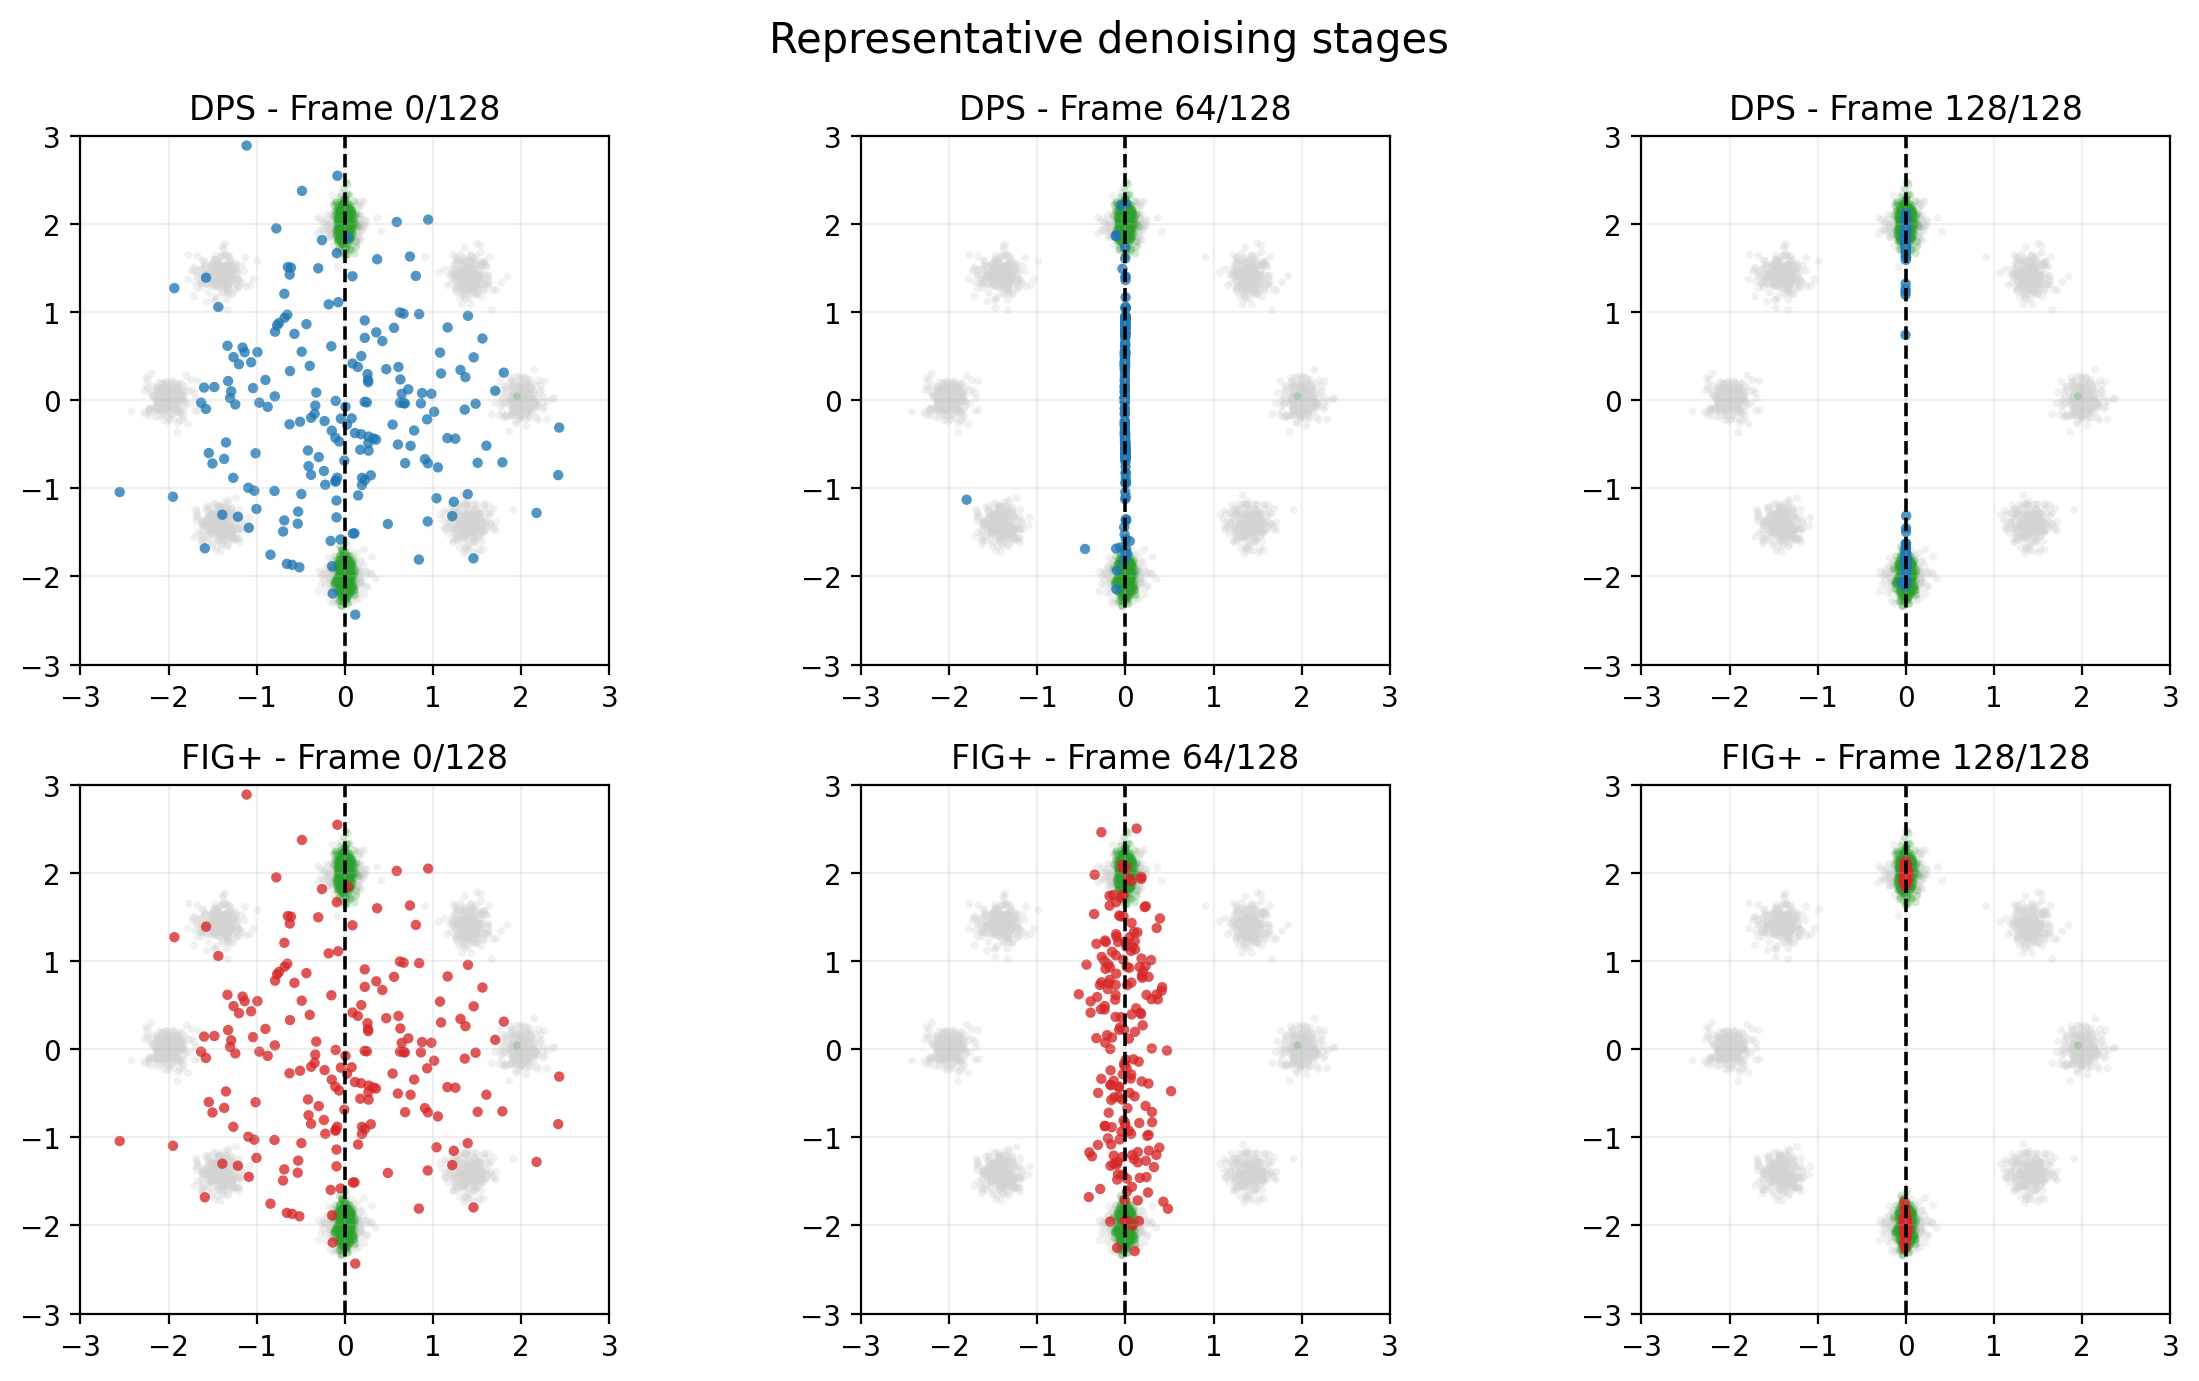
\includegraphics[width=\textwidth]{animations/eight_gaussians_sigma_0.05_x1_p0.00_vs_dps_vs_fig_plus_strip.png}
        \caption{Eight-Gaussians, fixed line \(x_1 = 0\).}
    \end{subfigure}
    \hfill
    \begin{subfigure}{0.49\textwidth}
        \centering
        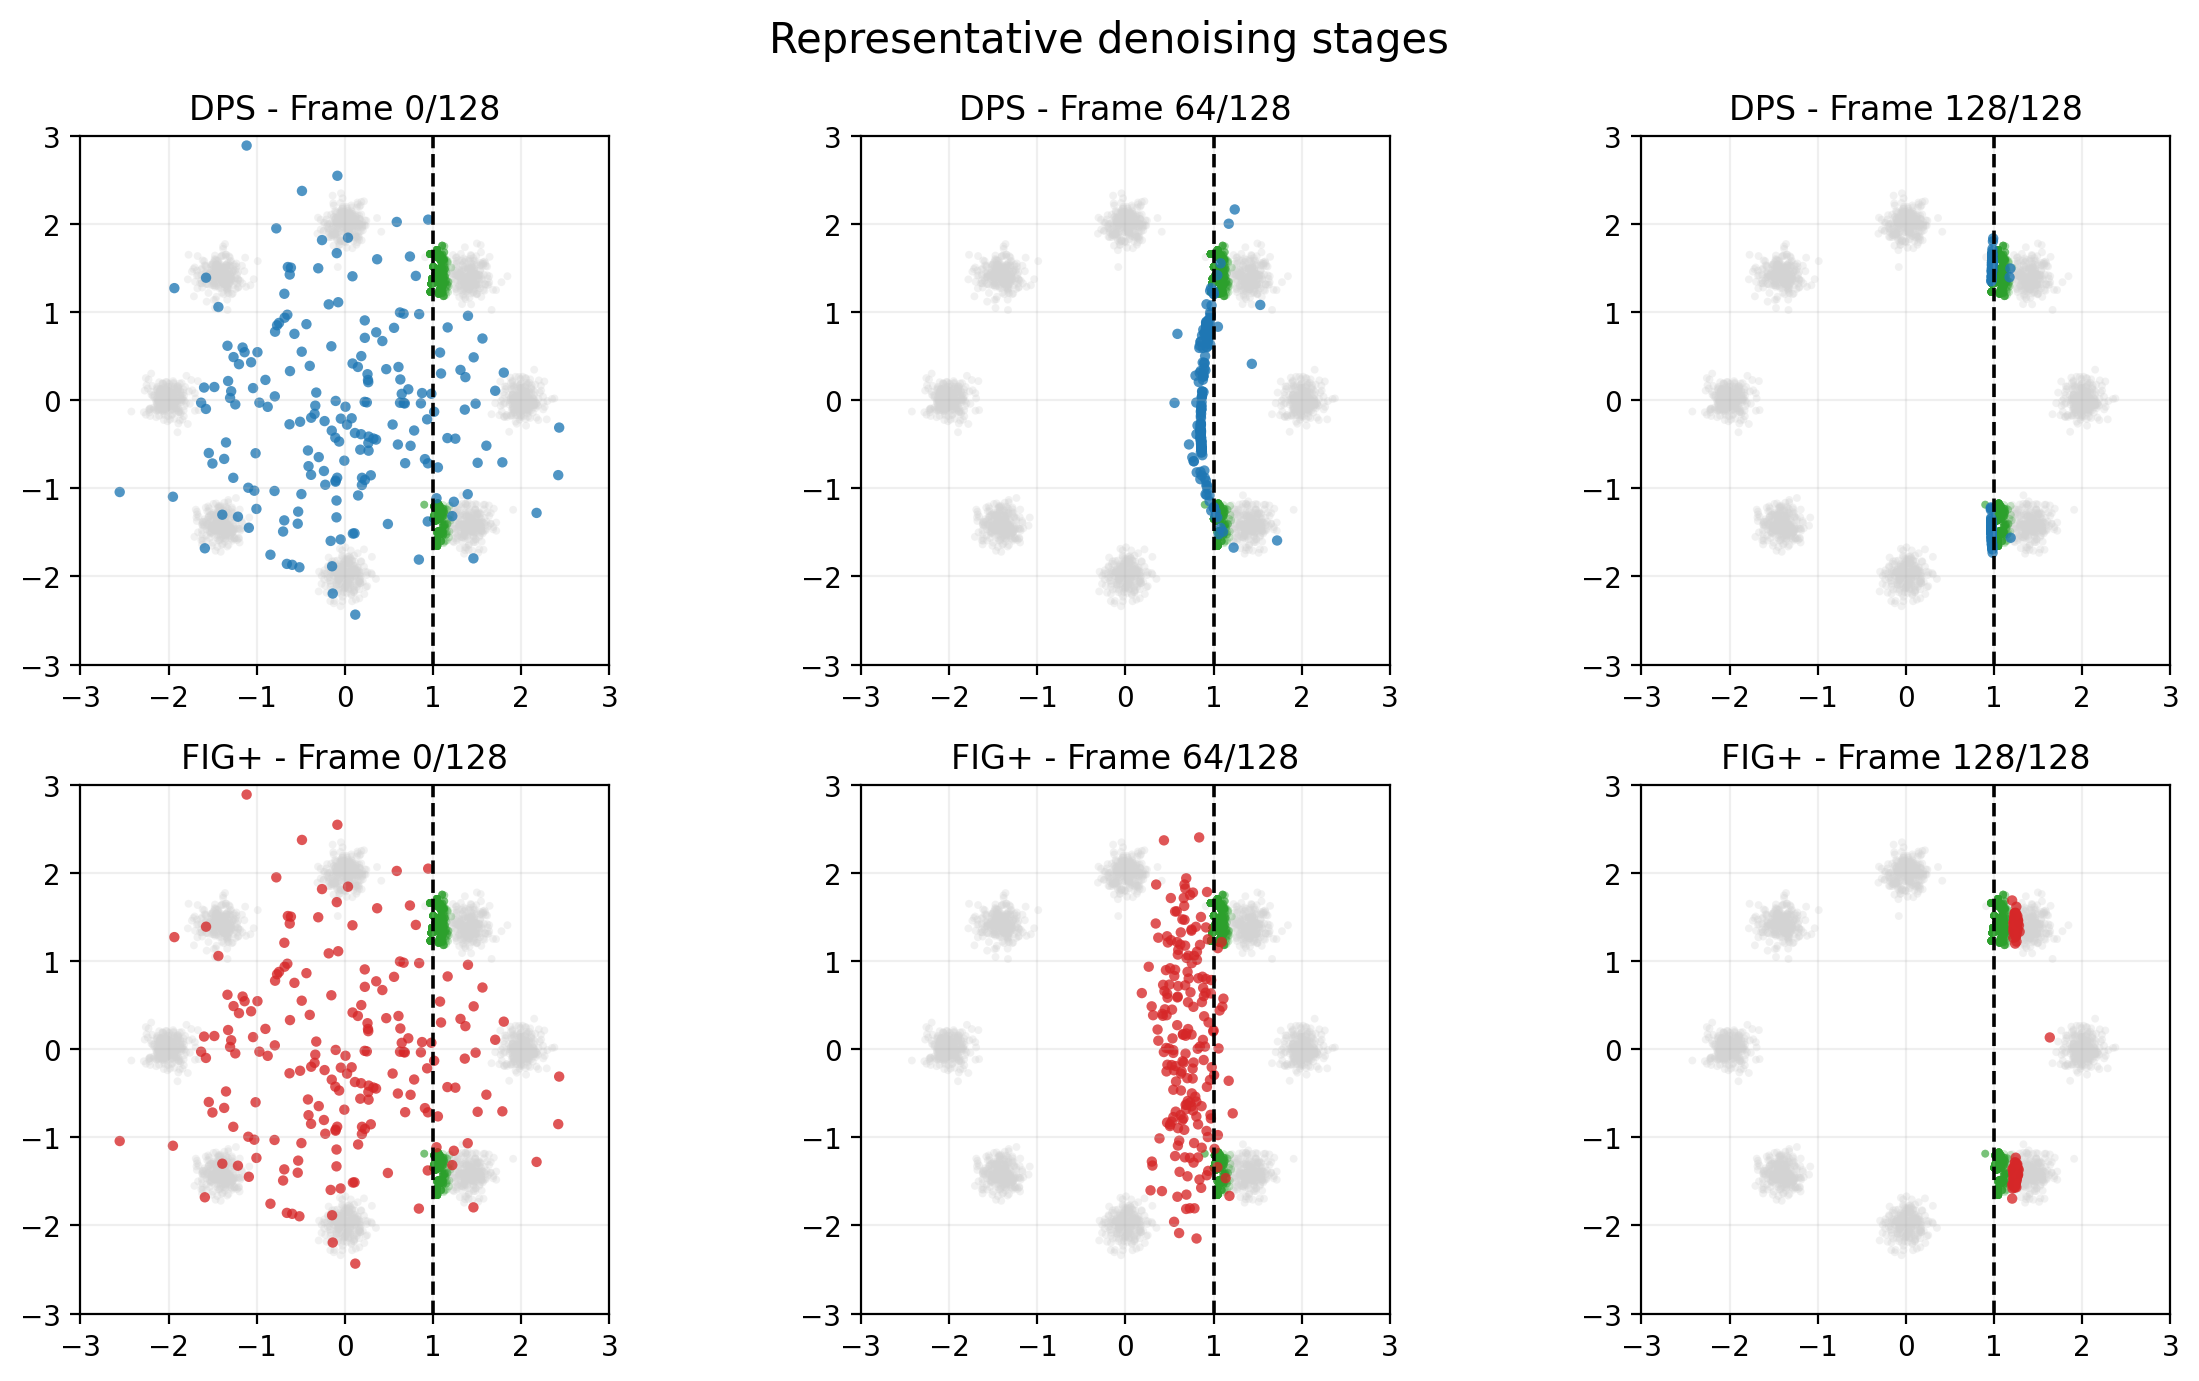
\includegraphics[width=\textwidth]{animations/eight_gaussians_sigma_0.05_x1_p1.00_vs_dps_vs_fig_plus_strip.png}
        \caption{Eight-Gaussians, fixed line \(x_1 = 1\).}
    \end{subfigure}
    \caption{Representative denoising stages for Eight-Gaussians. The two visible posterior modes correspond to the two clusters compatible with the observed \(x_1\). FIG+ remains concentrated around those modes, while DPS can overshoot or keep unnecessary spread before convergence.}
    \label{fig:eight_dynamics}
\end{figure*}

These fixed-line experiments are especially helpful for understanding the inpainting interpretation of the task. The first coordinate is observed, the second is hidden, and the solver must reconstruct the distribution of plausible hidden coordinates conditioned on the observation. In this view, “landing on the line” is necessary but not sufficient: the real goal is to place mass at the correct modes \emph{along} the line. The figures above show that FIG+ is much better at this than plain FIG and, in the present configuration, more stable than DPS.

The full animations are available alongside the paper at
\begin{center}
\texttt{animations/two\_moons\_sigma\_0.05\_x1\_p0.00\_vs\_dps\_vs\_fig\_plus.gif} \\
\texttt{animations/two\_moons\_sigma\_0.05\_x1\_p1.00\_vs\_dps\_vs\_fig\_plus.gif} \\
\texttt{animations/eight\_gaussians\_sigma\_0.05\_x1\_p0.00\_vs\_dps\_vs\_fig\_plus.gif} \\
\texttt{animations/eight\_gaussians\_sigma\_0.05\_x1\_p1.00\_vs\_dps\_vs\_fig\_plus.gif}
\end{center}

\section{Discussion}

Several conclusions emerge from the final benchmark.

\paragraph{1. The prior architecture matters.}
The original plain MLP was too weak for Eight-Gaussians and could visually understate the true quality of the learned prior. The residual, time-conditioned denoiser with EMA changes that regime completely: the unconditional fit is now strong enough that the conditional results are primarily about the solver, not about prior failure.

\paragraph{2. FIG+ is the most reliable conditional sampler in this setting.}
Across both datasets and all tested noise levels, FIG+ achieves the best posterior mean MSE and the best SWD. This confirms that the Tweedie-style reinjection of the hidden coordinate is crucial when the observation behaves like a mask.

\paragraph{3. Plain FIG remains too brittle for the present operator.}
Even when its measurement MSE is not catastrophic, plain FIG often misses the posterior geometry. The issue is not only whether the line constraint is enforced, but whether the solver preserves the correct multimodal distribution along that line.

\paragraph{4. DPS is strong but hyperparameter-sensitive.}
With the improved prior, DPS remains competitive in some regimes, especially on Eight-Gaussians at moderate and high measurement noise. However, the fixed guidance strength used here is clearly not robust across all posterior geometries. This is visible in the sharp failure cases at Two-Moons \(\sigma_n=0.5\) and Eight-Gaussians \(\sigma_n=0.05\).

\paragraph{5. The toy-2D setting remains highly informative.}
The benchmark makes posterior geometry directly visible. One can see when a solver merely satisfies the measurement and when it actually reconstructs the correct conditional distribution. This interpretability is the main value of the toy benchmark.

\section{Limitations and Future Work}

The current paper focuses on a deliberately minimal setting. Several extensions would be natural:
\begin{itemize}[leftmargin=1.5em]
    \item retuning DPS guidance strength as a function of the prior and measurement noise;
    \item larger evaluation sweeps with more test observations and more reference samples;
    \item additional linear operators, including rotated projections and full-rank noisy maps;
    \item nonlinear observation models;
    \item a direct bridge from the toy benchmark back to the image-scale operators of the original FIG repository.
\end{itemize}

These directions would help separate which phenomena are generic properties of the solver and which are specific to the present mask-like inverse problem.

\section{Conclusion}

This work transforms the original FIG repository into a complete toy-2D benchmark for inverse problems. The final version of the benchmark includes stronger residual DDPM priors, EMA sampling, refreshed quantitative evaluations, and fixed-line denoising animations that expose the conditional dynamics directly. With this improved setup, the conclusion is clear: FIG+ is the most effective method overall on posterior-quality metrics, plain FIG remains fragile, and DPS is competitive but sensitive to guidance tuning. More broadly, the study shows why toy benchmarks are valuable: they expose the geometry of conditional generation directly and make algorithmic behavior observable rather than merely measurable.

\section*{Practical Note}

No LaTeX engine was available on the current machine at generation time, so this source is provided ready to compile, together with all figures and animation assets referenced above.

\end{document}
